\paragraph[QuizziPedia::Front-End::Controllers\\::QuestionsManagementController]{QuizziPedia::Front-End::Controllers::QuestionsManagementController}
\begin{figure} [ht]
	\centering
	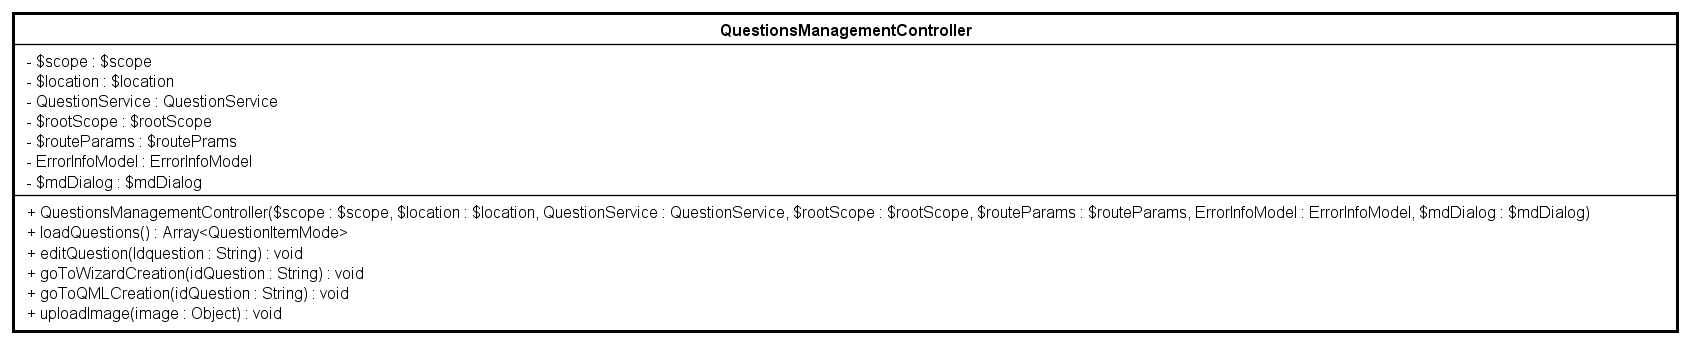
\includegraphics[scale=0.35]{UML/Classi/Front-End/QuizziPedia_Front-end_Controller_QuestionsManagementController.png}
	\caption{QuizziPedia::Front-End::Controllers::QuestionsManagementController}
\end{figure} \FloatBarrier
\begin{itemize}
	\item \textbf{Descrizione}: questa classe permette di gestire le domande create dall'utente e di crearne di nuove;
	\item \textbf{Utilizzo}: fornisce le funzionalità per richiedere al \textit{server\ped{G}} le domande create dall'utente e mostrarle nella pagina dedicata. Inoltre permette di catturare gli eventi per modificare le domande esistenti e per crearne una di nuova; 
	\item \textbf{Relazione con altre classi}:
	\begin{itemize}
		\item \textbf{IN \texttt{QuestionsManagementModelView}}: classe di tipo \textit{modelview\ped{G}} la cui istanziazione è contenuta all'interno della variabile di ambiente \$scope di \textit{Angular\ped{G}}. All'interno di essa sono presenti le variabili e i metodi necessari per il \textit{Two-Way Data-Binding\ped{G}} tra la \textit{view\ped{G}} \texttt{QuestionsManagementView} e il \textit{controller\ped{G}} \texttt{QuestionsManagementController}; 
		\item \textbf{IN \texttt{QuestionService}}: questa classe permette di ottenere domande esistenti e salvare nuove domande;
		\item \textbf{IN \texttt{QuestionsService}}: questa classe permette di ottenere domande esistenti e salvare nuove domande.
	\end{itemize}
	\item \textbf{Attributi}:
	\begin{itemize}
		\item \texttt{-} \texttt{\$scope: \$scope} \\
		Campo dati contenente un riferimento all'oggetto \$scope creato da \textit{Angular\ped{G}}, viene utilizzato come mezzo di comunicazione tra il \textit{controller\ped{G}} e la \textit{view\ped{G}}. Contiene gli oggetti che definiscono il \textit{model\ped{G}} dell'applicazione;
		\item \texttt{-} \texttt{\$location: \$location} \\
		Campo dati contenente un riferimento al servizio creato da \textit{Angular\ped{G}} che permette di accedere alla barra degli indirizzi del \textit{browser\ped{G}}, i cambiamenti all'URL nella barra degli indirizzi si riflettono in questo oggetto e viceversa;
		\item \texttt{-} \texttt{QuestionService: QuestionsService}\\
		Campo dati contenente un riferimento al servizio che si occupa della gestione delle informazioni legate alle domande;
		\item \rootscopeA;
		\item \routeparamsA;
		\item \errorinfomodelA;
		\item \mddialogA.
	\end{itemize}
	\item \textbf{Metodi}:
	\begin{itemize}
		\item \texttt{+} \texttt{QuestionsManagementsController(\$scope: \$scope, \$location: \$location, QuestionService: QuestionService, \$rootScope: \$rootScope, \$routeParams: \$routeParams, ErrorInfoModel: ErrorInfoModel, \$mdDialog: \$mdDialog)} \\ 
		Metodo costruttore della classe. \\
		\textbf{Parametri}:
		\begin{itemize}
			\item \texttt{\$scope: \$scope} \\
			Parametro contenente un riferimento all'oggetto \$scope creato da \textit{Angular\ped{G}}. Viene utilizzato come mezzo di comunicazione tra il \textit{controller\ped{G}} e la \textit{view\ped{G}}. Contiene gli oggetti che definiscono il \textit{viewmodel\ped{G}} e il \textit{model\ped{G}} dell'applicazione;
			\item \texttt{\$location: \$location} \\
			Parametro contenente un riferimento al servizio creato da \textit{Angular\ped{G}} che permette di accedere alla barra degli indirizzi del \textit{browser\ped{G}}, i cambiamenti all'URL nella barra degli indirizzi si riflettono in questo oggetto e viceversa;
			\item \texttt{QuestionService: QuestionService} \\
			Parametro contenente un riferimento al servizio che si occupa della gestione delle informazioni legate alle domande;
			\item \rootscopeP;
			\item \routeparamsP;
			\item \errorinfomodelP;
			\item \mddialogP. 
		\end{itemize}
		\item \texttt{-} \texttt{loadQuestions() : Array<QuestionItemMode>} \\ 
		Metodo che acquisisce le domande create dall'utente attraverso il \texttt{QuestionService};\\
		\item \texttt{+} \texttt{editQuestion(idQuestion: String) : void} \\ 
		Metodo che gestisce l'evento click sul pulsante per modificare la domanda. Effettua il redirect alla pagina di modifica della domanda. \\
		\textbf{Parametri}:
		\begin{itemize}
			\item \texttt{idQuestion: String} \\
			Parametro contenente l'id della domanda da modificare.
		\end{itemize}
				
		\item \texttt{+} \texttt{goToWizardCreation(idQuestion: String) : void} \\ 
		Metodo che gestisce l'evento click sul pulsante per creare una domanda. Effettua il redirect alla pagina di creazione della domanda con wizard; \\
		\item \texttt{+} \texttt{goToQMLCreation(idQuestion: String) : void} \\ 
		Metodo che gestisce l'evento click sul pulsante per creare una domanda. Effettua il redirect alla pagina di creazione della domanda con editor QML;\\
		\item \texttt{+} \texttt{uploadImage(image: Object) : void} \\ 
		Metodo che gestisce l'evento caricare un'immagine. \\
		\textbf{Parametri}:
		\begin{itemize}
			\item \texttt{image: Object} \\
			Parametro contenente un'immagine.
		\end{itemize}
	\end{itemize}
\end{itemize}

